%%%%%%%%%%%%%%%%%%%%%%%%%%%%%%%%%%%%%%%%%%%%%%%%%%%%%%%%%%%%%%%%%%%%%%
% amspaper.tex --  LaTeX2e-based template for submissions to American 
% Meteorological Society Journals, including
%
% JAS 	-- Journal of the Atmospheric Sciences
% JAMC 	-- Journal of Applied Meteorology and Climatology
% JPO 	-- Journal of Physical Oceanography
% MWR 	-- Monthly Weather Review
% JTECH -- Journal of Atmospheric and Oceanic Technology
% WAF 	-- Weather and Forecasting
% JCLI 	-- Journal of Climate
% JHM 	-- Journal of Hydrometeorology
% JAM 	-- Journal of Applied Meteorology
%
% Template developed by B. Papa and S. Cooley, AMS. 
% Email questions to latex@ametsoc.org.
%
% August 12, 2008 (SRC)
%	- Clarified/added header notes, comments throughout
%	- Improved title page
%	- Edited text of document for clarity
%	- Altered list styles to adhere to AMS style, added comments
%	- Removed incorrect commands (i.e., \catcode) (corrects umlaut bug)
%	- Moved non-template commands to ametsoc.sty
%
% August, 2008 - B. Papa
% - Updated to handle two column journal page output
% - Updated text with new/modified instructions
%
%%%%%%%%%%%%%%%%%%%%%%%%%%%%%%%%%%%%%%%%%%%%%%%%%%%%%%%%%%%%%%%%     
%%%%%%%%%%%%%%%%%%%%%%%%%%%%%%%%%%%%%%%%%%%%%%%%%%%%%%%%%%%%%%%%
%																															 %
%				USE THIS TEMPLATE, AMETSOC.STY, AND AMETSOC.BST				 %
%			        OR YOUR TEX FILES WILL NOT BE USED				  		 %
%																															 % 
%%%%%%%%%%%%%%%%%%%%%%%%%%%%%%%%%%%%%%%%%%%%%%%%%%%%%%%%%%%%%%%%
%%%%%%%%%%%%%%%%%%%%%%%%%%%%%%%%%%%%%%%%%%%%%%%%%%%%%%%%%%%%%%%%

%%%%%%%%%%%%%%%%%%%%%%%%%%%%%%%%%%%%%%%%%%%%%%%%%%%%%%%%%%%%%%%%%%%%%
% PREAMBLE
%%%%%%%%%%%%%%%%%%%%%%%%%%%%%%%%%%%%%%%%%%%%%%%%%%%%%%%%%%%%%%%%%%%%%
%
% The following two commands will generate a PDF that follows all the requirements for submission
% and peer review.  Uncomment these commands to generate this output (and comment out the two lines below.)
%
% DOUBLE SPACE VERSION FOR SUBMISSION TO THE AMS
\documentclass[12pt]{article}
\usepackage{ametsoc}
\linenumbers
%
% The following two commands will generate a single space, double column paper that closely
% matches an AMS journal page.  Uncomment these commands to generate this output (and comment
% out the two lines above. FOR AUTHOR USE ONLY. PAPERS SUBMITTED IN THIS FORMAT WILL BE RETURNED
% TO THE AUTHOR for submission with the correct formatting.
%
% TWO COLUMN JOURNAL PAGE LAYOUT FOR AUTHOR USE ONLY
%\documentclass[10pt]{article}
%\usepackage{ametsoc2col}
\usepackage{subfigure}
\usepackage{comment}
\usepackage{verbatim}
\usepackage{fancyvrb}

%
%%%%%%%%%%%%%%%%%%%%%%%%%%%%%%%%%%%%%%%%%%%%%%%%%%%%%%%%%%%%%%%%%%%%%
% ABSTRACT
%
% Enter your Abstract here
%%%%%%%%%%%%%%%%%%%%%%%%%%%%%%%%%%%%%%%%%%%%%%%%%%%%%%%%%%%%%%%%%%%%%
\newcommand{\myabstract}{The authors propose a new technique for parallelizations of tangent linear and adjoint codes, which were applied in the redevelopment for the Weather Research and Forecasting (WRF) Model with its Advanced Research WRF dynamic core using the automatic differentiation engine. The tangent linear and adjoint codes of the WRF model (WRFPLUS) now has the following improvements: 
\begin{itemize}
\item A complete check interface ensures that developers write the tangent linear and adjoint codes in accuracy with ease and efficiency.
\item To parallelize the WRFPLUS model, the authors adopted a new technique based on the nature of duality that existed among Message Passing Interface communication routines. The Registry in the WRF model was extended to automatically generate the tangent linear and adjoint codes of the required communication operations. This approach dramatically speeds up the software development cycle of the parallel tangent linear and adjoint codes and leads to improved parallel efficiency. 
\item Module interfaces were constructed for coupling tangent linear and adjoint codes of the WRF model with  applications such as four-dimensional variational data assimilation, forecast sensitivity to observation and other.
\end{itemize}
 }
%
\begin{document}
%
%%%%%%%%%%%%%%%%%%%%%%%%%%%%%%%%%%%%%%%%%%%%%%%%%%%%%%%%%%%%%%%%%%%%%
% TITLE
%
% Enter your TITLE here
%%%%%%%%%%%%%%%%%%%%%%%%%%%%%%%%%%%%%%%%%%%%%%%%%%%%%%%%%%%%%%%%%%%%%
\title{\textbf{\large{Development of the Upgraded Tangent Linear and Adjoint of the Weather Research and Forecasting (WRF) Model}}}
%
% Author names, with corresponding author information. 
% [Update and move the \thanks{...} block as appropriate.]
%
\author{\textsc{Xin Zhang}
				\thanks{\textit{Corresponding author address:} 
				Dr. Xin Zhang, NCAR, MMM, P.O. Box 3000, 
				 Boulder, CO 80307. 
				\newline{E-mail: xinzhang@ucar.edu}}\\
\textit{\footnotesize{National Center for Atmospheric Research, Boulder, Colorado 80307, USA}}
\and 
\centerline{\textsc{Xiang-Yu Huang}}\\% Add additional authors, different institution
\centerline{\textit{\footnotesize{National Center for Atmospheric Research, Boulder, Colorado 80307, USA}}}
\and
\centerline{\textsc{Ning Pan}}\\% Add additional authors, different institution
\centerline{\textit{\footnotesize{Fujian Meteorological Bureau, Fuzhou, Fujian, China}}}
}
%
% The following block of code will handle the formatting of the title page depending on whether
% we are formatting a double column (dc) author draft or a single column paper for submission.
% AUTHORS SHOULD SKIP OVER THIS... There is nothing to do in this section of code.
\ifthenelse{\boolean{dc}}
{
\twocolumn[
\begin{@twocolumnfalse}
\amstitle

% Start Abstract (Enter your Abstract above.  Do not enter any text here)
\begin{center}
\begin{minipage}{13.0cm}
\begin{abstract}
	\myabstract
	\newline
	\begin{center}
		\rule{38mm}{0.2mm}
	\end{center}
\end{abstract}
\end{minipage}
\end{center}
\end{@twocolumnfalse}
]
}
{
\amstitle
\begin{abstract}
\myabstract
\end{abstract}
\newpage
}
%%%%%%%%%%%%%%%%%%%%%%%%%%%%%%%%%%%%%%%%%%%%%%%%%%%%%%%%%%%%%%%%%%%%%
% MAIN BODY OF PAPER
%%%%%%%%%%%%%%%%%%%%%%%%%%%%%%%%%%%%%%%%%%%%%%%%%%%%%%%%%%%%%%%%%%%%%
%
\section{Introduction}

During the past two decades, the use of the adjoint technique in meteorology and oceanography rapidly increased.  The adjoint model is a powerful tool in many applications, such as data assimilation, parameter estimation, and sensitivity analysis. (\cite{Errico1992}; \cite{Errico1997}; \cite{Rabier1996}; \cite{Langland1999}; \cite{Li1999}; \cite{Xiao2002}; \cite{Xiao2008}; \cite{Kleist2005a}; \cite{Kleist2005b})

The Weather Research and Forecasting (WRF) Modeling System (\cite{Skamarock2008}) is a multi-agency effort to provide a next-generation mesoscale forecast model and data assimilation system that will advance both the understanding and the prediction of mesoscale weather as well as accelerate the transfer of research advances into operations. The WRF model was designed to be an efficient massively parallel computing code to take advantage of advanced high-performance computing systems. The code, which can be configured for both research and operations, also offers numerous physics options. The WRF model is maintained and supported as a community model to facilitate wide use internationally, for research, operations, and teaching. The model is suitable for a broad span of applications across scales ranging from large-eddy to global simulations. Such applications include real-time numerical weather prediction, data assimilation development and studies, parameterized-physics research, regional climate simulations, air-quality modeling, atmosphere-ocean coupling, and idealized simulations. As of this writing, the WRF model is in operational and research use around the world, and the number of registered WRF users exceeds 20000.

The first version of the adiabatic WRF tangent linear model (TLM) and adjoint model (ADM) system (WAMS) was developed by National Center for Atmospheric Research (NCAR) around 2007 (\cite{Xiao2008}). The WAMS is used in the adjoint sensitivity analysis (\cite{Xiao2008}) and Four-Dimensional Variational Data Assimilation (4D-Var) (\cite{Huang2009}). It took us more than one year to complete the parallelization of the WAMS by following the traditional incremental and iteraive parallelization procedures, which include algorithm analysis, identifying the time-consuming hotspot, data dependency analysis, locating the halo exchange and manually writing the communication routines for data exchanging. In the past few years, due to the tremendous time required for hand-coding parallellization, the WAMS has failed to repeat the rapid development pattern of the WRF model and the WRF Data Assimilation System (WRFDA)(\cite{Barker2012}). The growing gap between the WAMS and the WRF/WRFDA makes the WAMS inconvenient to use with other systems. One example was that the WRF 4D-Var system could not read the WRF boundary conditions of later versions because the WAMS was left behind and it does not  include the upgrades of the boundary condition data structure in the WRF. Furthermore, because the WAMS uses the disk input/output (I/O) for storing/reading basic states trajectory and exchanging data among the FWM, TLM and ADM, the parallel efficiency is unsatisfactory on modern high-performance computers with distributed memory parallelization, especially for 4D-Var applications.  
 
Encouraged by the rapid developments of  4D-Var, cloud analysis, forecast sensitivity to observations and chemistry data assimilation, we redeveloped the WRF TLM and ADM (called WRFPLUS) based on the latest repository WRF. Compared with the WAMS developed by \cite{Xiao2008} and \cite{Huang2009}, the new system is an all-in-one system which includes the WRF full-physics forward model (FWM), TLM and ADM; This system also includes the tangent linear check and adjoint check procedures. A set of module interfaces was developed for easily coupling the WRFPLUS model with other systems such as data assimilation and adjoint sensitivity applications.  An new approach was applied to develop the parallel code that dramatically reduces the software development cycle of the parallel TLM and ADM; and the derived parallel TLM and ADM have better parallel efficiency compared to the FWM.

The purpose of this paper is to describe the technical aspects of the newly developed WRFPLUS model. A brief introduction of the development of the WRFPLUS model is presented in section 2, followed by a demonstration of the linearity and adjoint tests in section 3. A detailed description of parallelization strategy for  tangent linear and adjoint codes, with the demonstated parallel performance are in section 4. Section 5 introduces the module interfaces constructed in the WRFPLUS model for coupling purposes, such as in WRF 4D-Var. Concluding remarks appear in section 6.

\section{Description of the WRF tangent linear and adjoint models}

After the release of the WRF model version 3.2, we started to use TAPENADE (\cite{Hascoet2004T2u}) to redevelop the TLM and the ADM of the WRF Advanced Research WRF (ARW) core based on the latest WRF model. The development of WRFPLUS model follows the same three phases proposed by \cite{Xiao2008}. First, numerical experiments were conducted to make sure that the adiabatic version of the WRF model with simplified physics paramterization routines can produce the major features that the full-physics model does. Second, the TLM and its ADM were generated by TAPENADE and modified manually whenever necessary. The third step was to verify the correctness of the TLM and the ADM.

TAPENADE is a source-to-source automatic differentiation (AD) tool for programs written in Fortran 77-95, i.e., TAPENADE generates a TLM or an ADM from the source code of a given model. Like other AD tools, TAPENADE struggles with such complicated codes as WRF�s third-order Runge-Kutta large timesteps and small acoustic timesteps (\cite{Xiao2008}).  Checking and improving TAPENADE-generated code can necessitate manual intervention (i) to represent first-order physical effects on the model evolution, (ii) to minimize code length so that developing its adjoint is simple, and (iii) to allow the code to run quickly in the iterations required to lower costs.  We also adopted three simplified physics packages that have maximum impact on a forecast compared to a no-physics model: surface friction, cumulus parmeterization, and large-scale condensation. These were developed by Jimy Dudhia (2012, personal communication) and are similar to the physics packages in the WAMS (\cite{Xiao2008}).

\section{Linearity test and adjoint test}

Testing TLM consistency with FWM as well as ADM consistency with TLM before either is used in any real application is essential (\cite{Vukicevic1991}; \cite{Errico1992}; \cite{Gilmour2001}). We developed the tangent linear and adjoint check procedures following \cite{Navon1992}.

Let $\mathbf{f}(\mathbf{x})$, $g\_\mathbf{f}(\mathbf{x},g\_\mathbf{x})$ and $a\_\mathbf{f}(\mathbf{x},a\_\mathbf{x})$ denote a FWM, a TLM and an ADM, respectively, where $\mathbf{x}$, $g\_\mathbf{x}$ and $a\_\mathbf{x}$ is the column vector of model state variables, perturbations of state variables and adjoint of state variables, respectively. The correctness of the TLM can be tested as:
\begin{equation}
\label{tlcheckf}
{\Phi(\lambda)}={\frac{\|\mathbf{f}(\mathbf{x}+{\lambda}g\_\mathbf{x})-\mathbf{f}(\mathrm{x})\|}{{\|g\_\mathbf{f}(\mathbf{x},{\lambda}g\_\mathbf{x})\|}}},  \lim_{\lambda \rightarrow 0}{\Phi(\lambda)}=1
\end{equation}
where $\|\|$ denotes the norm of the vector.
The adjoint relation is tested by :
\begin{equation}
\label{adcheck}
\langle g\_\mathbf{f}(\mathbf{x},g\_\mathbf{x}),g\_\mathbf{f}(\mathbf{x},g\_\mathbf{x}) \rangle = \langle a\_\mathbf{f}(\mathbf{x},g\_\mathbf{f}(\mathbf{x},g\_\mathbf{x})),g\_\mathbf{x} \rangle
\end{equation}
If the tangent linear and adjoint codes are correct, the above two relations should hold up to the machine accuracy. Because different model variables have different magnitudes, we also designed the capability to perform checks on individual variables separately. We performed the tangent linear and adjoint checks with the test case being integrated up to 24h. We sequentially reduced the initial perturbations by a factor ($\lambda$) of $10$ and repeatedly calculated $\Phi(\lambda)$ in Eqs. (\ref{tlcheckf}) on NCAR's IBM machine with 64-bit precision. Table \ref{tlcheck} shows the value of $\Phi(\lambda)$ from the tangent linear forecasts and the differences between two nonlinear forecasts over the whole domain. This indicated that the tangent linear forecast approximates the difference between two nonlinear forecasts as the initial perturbations decrease and approach zero.

In the adjoint relationship, the left-hand side (lhs) involves only the tangent linear code, while the right-hand side (rhs) involves the adjoint code. If lhs and rhs have the same value with machine accuracy, the adjoint code is correct compared with the tangent linear code. Using the same test case with 24h integration, lhs and rhs for the test case are 0.14182720729878E+14 and 0.14182720729883E+14, respectively. This indicates that the adjoint code is correct.


\section{Parallelization of the WRFPLUS model}

TAPENADE has few problems in generating tangent linear and adjoint codes from the sequential forward codes. However, it cannot derive such codes of parallel communication routines inside a parallel forward model. In most of the atmospheric and oceanic models, the communication routines to parallelize finite difference algorithms are linear operators; hence as matrices, the adjoint is simply the transpose, which is the dual operator, and the tangent linear is the original linear operator acting on the perturbations (see \cite{Cheng2006ADb} and \cite{Utke2009TAM}). With the proper coding structure and available parallel communication routines in forward codes, it is straightforward to write communication routines for tangent linear models. We  need only use the same parallel communication templates in forward codes and add the corresponding perturbation variables. In the adjoint code, the data flow of the original program needs to be reversed and any communication needs to be reversed as well. Due to the duality between $MPI\_ SEND$ and $MPI\_ RECV$ calls, in transforming FWM to ADM, we replace $MPI\_ SEND$ calls with $MPI\_ RECV$, and vice versa. Please note that it is the adjoint variable which is subject to being exchanged in the ADM. Figures \ref{fig:fwm_mpi} and \ref{fig:adm_mpi} could be helpful to understand the data flow of communication in the FWM and the ADM, respectively. In the FWM, the variable $U$ in the ghost region of processor P1 will be overwritten by the value of $U$ received from processor P0. In the ADM, the communication needs to be reversed. The adjoint variable $a\_U$ in the ghost region of P1 will be sent to P0 and added to the value of $a\_U$ of P0; then the $a\_U$ in the ghost region of P1 will be set to zero. 

In the WRF model, hundreds of thousands of lines of code are automatically generated from a user-edited table called the Registry (\cite{John2004}).  The Registry provides a high-level single point of control over the fundamental structure of the model data.  It contains lists describing state data fields and their attributes:  dimensionality, binding to particular solvers, association with WRF I/O streams, communication operations, and run time configuration options (namelist elements and their bindings to model control structures).  Adding or modifying a state variable to WRF involves modifying a single line of a single file; this single change is then automatically propagated to scores of locations in the source code the next time the code is compiled.

Halo entries in the Registry define communication operations in the model. Halo entries specify halo updates around a patch horizontally. A typical halo entry is :
\begin{Verbatim}[frame=single]
halo      HALO_EM_C     dyn_em    4:u_2,v_2
\end{Verbatim}
The first field is the keyword "halo". The second entry --"HALO\_EM\_C", which is the given name of the halo exchange template, is used in the model to refer to the communication operation being defined. The third entry denotes the associated solver, and the fourth entry is a list of information about the operation. This example specifies that 4 points (one cell each in north, south, east, and west directions, respectively) of the stencil are used in updating the state arrays for fields $u\_2$ and $v\_2$ across the processors. During compilation, the WRF Registry automatically generates a code segment based on this halo entry: 
\begin{Verbatim}[frame=single]
...
CALL HALO_EM_C_sub ( grid, local_communicator, ...)
...
\end{Verbatim}
The code snippet is included in the places where the communications are needed. At the same time, the Registry also generates the subroutine "HALO\_EM\_C\_sub":
\begin{Verbatim}[frame=single]
...
! for Y direction
CALL RSL_LITE_PACK ( local_communicator, grid%u_2, ...,0,...
CALL RSL_LITE_PACK ( local_communicator, grid%v_2, ...,0,...
CALL RSL_LITE_EXCH_Y
CALL RSL_LITE_PACK ( local_communicator, grid%u_2, ...,1,...
CALL RSL_LITE_PACK ( local_communicator, grid%v_2, ...,1,...
...
! for X direction
CALL RSL_LITE_PACK ( local_communicator, grid%u_2, ...,0,...
CALL RSL_LITE_PACK ( local_communicator, grid%v_2, ...,0,...
CALL RSL_LITE_EXCH_X
CALL RSL_LITE_PACK ( local_communicator, grid%u_2, ...,1,...
CALL RSL_LITE_PACK ( local_communicator, grid%v_2, ...,1,...
...
\end{Verbatim}
In the above code segment, the outgoing slices of $u\_2$ and $v\_2$ for Y direction (south-north) exchanging are packed by "RSL\_LITE\_PACK" into a local contiguous memory region. Therefore, one call of "RSL\_LITE\_EXCH\_Y" is able to complete the data exchanges in the south-north direction. Once every processor receives the incoming data, "RSL\_LITE\_PACK" will be called again with different arguments to unpack the data to the ghost area position. The similar operations are performed in the X direction (east-west) as well.

The forward communication codes show an efficient chain of established relationships. Therefore, perturbing and adjointing the code is simple. However, it is an error-prone and time-consuming task to manually write all tangent linear and adjoint codes of communication subroutines. Since the WRF Registry is able to generate halo exchange routines, there is the possibility of letting the Registry generate the tangent linear and adjoint codes of halo exchanges too. To enable the WRF Registry to generate the corresponding tangent linear and adjoint communication codes automatically, we modified the Registry and added a new entry "halo\_nta" as:
\begin{Verbatim}[frame=single]
halo_nta      HALO_EM_C     dyn_em     4:u_2,v_2
\end{Verbatim}
With this new entry, the Registry will not only generate "HALO\_EM\_C\_sub", but also generate "HALO\_EM\_C\_TL\_sub" for tangent linear codes and "HALO\_EM\_C\_AD\_sub" for adjoint codes. The subroutine "HALO\_EM\_C\_TL\_sub" looks like:
\begin{Verbatim}[frame=single]
...
! for Y direction
CALL RSL_LITE_PACK ( local_communicator, grid%u_2, ...,0,...
CALL RSL_LITE_PACK ( local_communicator, grid%v_2, ...,0,...
CALL RSL_LITE_PACK ( local_communicator, grid%g_u_2, ...,0,...
CALL RSL_LITE_PACK ( local_communicator, grid%g_v_2, ...,0,...
CALL RSL_LITE_EXCH_Y
CALL RSL_LITE_PACK ( local_communicator, grid%u_2, ...,1,...
CALL RSL_LITE_PACK ( local_communicator, grid%v_2, ...,1,...
CALL RSL_LITE_PACK ( local_communicator, grid%g_u_2, ...,1,...
CALL RSL_LITE_PACK ( local_communicator, grid%g_v_2, ...,1,...
...
! for X direction
\end{Verbatim}
The TLM has exactly the same exchange stencil and data flow as the FWM; however, in addition to the basic state fields ($u\_2$ and $v\_2$), the perturbation fields ($g\_u\_2$ and $g\_v\_2$) exchanged as well, which is required by the TLM.
 
The adjoint code "HALO\_EM\_C\_AD\_sub" looks like:
\begin{Verbatim}[frame=single]
...
! for Y direction
CALL RSL_LITE_PACK_AD ( local_communicator, grid%a_u_2, ...,0,...
CALL RSL_LITE_PACK_AD ( local_communicator, grid%a_v_2, ...,0,...
CALL RSL_LITE_EXCH_Y
CALL RSL_LITE_PACK_AD ( local_communicator, grid%a_u_2, ...,1,...
CALL RSL_LITE_PACK_AD ( local_communicator, grid%a_v_2, ...,1,...
...
! for X direction
\end{Verbatim}
The ADM also has the same exchange stencil as the FWM and the TLM, but the data flow is reversed. On each processor, the entire patch of basic state variables (including halo) is stored in the memory stack during the forward recomputation stage and will be restored from the memory stack during the adjoint calculation. Therefore, in adjoint communication codes, only the adjoint variables ($a\_u\_2$ and $a\_v\_2$) need to be exchanged and the new subroutines "RSL\_LITE\_PACK\_AD" will pack the data slices from where we receive data in the FWM and the TLM for sending and unpack the received data to the slices where we send out data in the FWM and the TLM. 

With the upgraded WRF Registry, all tangent linear and adjoint communication routines are generated automatically during compilation. To manually insert the tangent linear and adjoint communication interfaces into the TLM and the ADM is straightforward. In the TLM,  the tangent linear communication routines are inserted into the same locations where the forward communication routines reside in the FWM. In the ADM, the calling sequence of the adjoint communication routines is the reverse of that in the FWM and the TLM. From the code snippets presented above, we found that because both basic state variables and perturbation variables are packed together, although the amount of data to communicate is doubled in the TLM, the communication latency is kept the same as in the FWM. This is highly desirable for a modern distributed memory parallel computer system with high bandwidth. In the ADM, in general, there are two stages: the first is the forward recomputation part, which propagates the basic states within one timestep and has the same communication latency and amount of data to communicate with the FWM; The second is the adjoint backward part, which has the same communication latency and amount as the first. Therefore, the total communication latency and amount of data to communicate are doubled in the ADM. However, due to the fact that the adjoint code may has three to four times the amount of computation code than the forward code and the computations to communications ratio is still large, the communication overhead is not substantial and should not impact the parallel scalability of the ADM.

\section{Parallel performance}

To demonstrate the parallel efficiency of the WRFPLUS model, we prepared the initial condition and boundary conditions for a 15km-resolution domain (not shown) with domain center at $32.6{^\circ}N$, $110{^\circ}E$ . There are $665\times383$ grid points in the horizontal direction and $45$ levels in the vertical direction; the timestep is $90s$. We tested this case on NCAR's two supercomputers: Lynx and Bluefire. Lynx is a single-cabinet Cray XT5m supercomputer, comprised of 76 compute nodes, each with 12 processors on 2 hex-core AMD 2.2 GHz Opteron chips, with a total of 912 processors. Each Lynx computer node has 16 gigabytes of memory, for 1.33 gigabytes per processor, and totaling 1.216 terabytes of memory in the system. Bluefire is an IBM clustered Symmetric MultiProcessing (SMP) system comprised of 4,096 Power 6 processors. The 4,096 processors are deployed in 128 nodes, each containing 32 processors. Nodes are interconnected with an InfiniBand switch for parallel processing using MPI. We used the default compilation options and the default processors topology calculated by the WRF model. We did not do any further optimization to get the best performance. Therefore, the following results do not reflect the best performance possible on a specific supercomputer.

We ran the WRFPLUS model on $16$, $32$, $64$, $128$, $256$, $512$, $1024$ and $2048$ processors of Bluefire and measured the parallel performance. Figure \ref{fig:bluefire} shows the results for the average wallclock time for one-timestep integration (Fig.\ref{fig:bf_a}) and speedup for the FWM, TLM and ADM, respectively (Fig.\ref{fig:bf_b}). Please note that the timing results for the FWM are different from the standard WRF run, which is compiled with 4 bytes-long real size. In the WRFPLUS, the FWM is compiled with 8 bytes long real size. In general, due to the higher precision requirement in the WRFPLUS, the actual computational performance of the FWM is slower than the standard WRF. Speedup for $N$ processors was calculated as the wallclock time using 16 processors divided by the wallclock time using $N$ processors. The computing times for all models are considerably reduced with an increased number of processors up to $2048$. In general, the TLM has a better speedup than the FWM and the ADM has a slightly better or comparable speedup than the FWM. The results confirm the successful implementation of the new parallel approach. 

We also ran the WRFPLUS model on $16$, $32$, $64$, $128$, $256$ and $512$ processors of Lynx and measured the parallel performance. Figure \ref{fig:lynx} shows the results for the average wallclock time for one-timestep integration (Fig.\ref{fig:lx_a}) and speedup (Fig.\ref{fig:lx_b}). We drew similar conclusions and again confirmed the high efficiency of the parallelization strategy of the WRFPLUS.

\section{Implementation of an inline coupling interface in the WRFPLUS model}

One of the motivations to upgrade the WRF TLM and ADM is to improve the computational performance of the WRF 4D-Var. The old WRF 4D-Var system contains a two-way coupling between the WRFDA and the WAMS (\cite{Huang2009}) exchanges information via disk files and is a multiple program multiple data (MPMD) system. During the coupling, the exchanged data are written to disk and a signal file is prepared to inform the other component that data is ready to be read. Exchange of a field between the WRFDA and the WAMS consists of gathering and scattering operations across the processors via disk files, which is vey inefficient on modern distributed-memory supercomputers with large number of processor. This limits the number of processors that can be used for high-resolution modeling.

Since the WRFDA and the WRFPLUS share the same software infrastructure including parallelization, field definition, I/O, Registry etc., it is straightforward to couple the WRFDA and the WRFPLUS to a single executable 4D-Var system, in which all information (basic states, perturbation and adjoint forcing) from the WRFPLUS is passed as arguments to the coupling interfaces and the WRFDA fetches the data from the coupling interfaces instead of disk files.

For this purpose, three major developments were needed:
\begin{enumerate}
        \item Enable the WRFPLUS model to be callable from the WRFDA with a simple application programming interface consisting of:
        \begin{enumerate}
		\item Initialize the WRFPLUS model. 
		\item Advance one of the WRFPLUS model components (FWM, TLM and ADM) . 
		\item Finalize the WRFPLUS model.
	\end{enumerate}
	\item Develop a set of regridding routines that can interpolate data on the WRFPLUS grid to the WRFDA grid (and vice-versa), which can be called by the WRFDA in full MPI parallel mode. 
	\item Modify the WRFDA to allow it to call the WRFPLUS with forcing data from the WRFDA and retrieve field data from the WRFPLUS (e.g. gradients).
\end{enumerate}
In this paper we  discuss only the first development, the other two developments will be introduced in a separate paper. 

The WRF model already has a well-defined routine that advances the integration, which makes calling it from an external model straightforward. New initialization and finalization routines had to be coded mostly to deal with the TLM and the ADM. A namelist option $dyn\_opt$ was borrowed to allow the WRFPLUS to decide which model will be advanced. $dyn\_opt=2$ will activate the FWM, $dyn\_opt=202$ will activate the TLM and   $dyn\_opt=302$ will activate the ADM.

The fully implemented interfaces as seen from the WRFDA point of view looks like this:
\fbox {
    \parbox{\linewidth}{
    \begin{itemize}
    	\item {\bf{Components routines :}} The  interfaces to activate forward, tangent linear and adjoint model
		\begin{itemize}
			\item {\bf{wrf\_run :}} Interface to run forward (nonlinear) model
			\item {\bf{wrf\_run\_tl :}} Interface to run tangent linear model
			\item {\bf{wrf\_run\_ad :}} Interface to run adjoint model
		\end{itemize}
	\item {\bf{Data exchange routines :}} The interfaces to exchange data between the WRFDA and the WRFPLUS
		\begin{itemize}
			\item {\bf{read\_xtraj :}} Read the trajectories from the FWM integration
			\item {\bf{save\_xtraj :}} Save the trajectories from the FWM integration
			\item {\bf{read\_tl\_pert :}} Read initial perturbation for the TLM  integration
			\item {\bf{save\_tl\_pert :}} Save trajectories of perturbation from the TLM integration.
			\item {\bf{read\_ad\_forcing :}} Read adjoint forcing for the ADM integration
			\item {\bf{save\_ad\_forcing :}} Save initial adjoint forcing from the ADM integration
		\end{itemize}
    \end{itemize}
        }
}
These interfaces are written not only for the coupling with the WRFDA but are designed for general coupling purposes. In addition to the coupling of the WRFDA and the WRFPLUS to construct the WRF 4D-Var, we successfully coupled the WRFPLUS with the community GSI to construct a GSI-based WRF 4D-Var (\cite{Zhang2013}). Figure \ref{fig:4dvar} shows the parallel performance of WRF 4D-Var run with 15km-resolution Continental U.S. (CONUS) domain (not shown), This domain has 450X450 horizontal grids and 51 vertical levels. The assimilation window is 6 hours and the integration timestep is 90s. Only GTS conventional data is assimilated. The WRF 4D-Var shows impressive scalability, i.e. with the addition of more processors, the total performance of the WRF 4D-Var increased accordingly. The implementation and coupling work quite well; it has already replaced the old WRF 4D-Var system since the V3.4 release of WRF 4D-Var. Beside the performance benefit, there are other advantages compared to the old WRF 4D-Var system. The execution of the new 4D-Var is simpler than before because it is unnecessary to launch a multiple program multiple data (MPMD) collection of different executables.  

\section{Conclusion}

In this paper we describe the implemented technique of the new tangent linear and adjoint codes of the WRF ARW core and demonstrated how, using TAPANADE (a free AD tool), the WRFPLUS was developed and carried forward into later versions. Compared to the WAMS, the new WRFPLUS has the following improvements: 1) The tangent linear and adjoint codes are maintained to be consistent with the latest WRF changes; 2) Parallelization strategy and efficiency are enhanced; 3) Complete tangent-linear and adjoint checks ensure the accuracy of the existing codes and newly developed codes; and 4) Module interfaces for coupling were constructed in the WRFPLUS that led to a single executable WRF 4D-Var system with efficient parallel performance and scalability.  


\section{Figures and tables}

\subsection{Figures}

%%%%%%%%%%%%%%%%%%%%%%%%%%%%%%%%%%%%%%%%%%%%%%%%%%%%%%%%%%%%%%%%%%%%%
% FIGURES
%%%%%%%%%%%%%%%%%%%%%%%%%%%%%%%%%%%%%%%%%%%%%%%%%%%%%%%%%%%%%%%%%%%%%
\begin{figure}[t]
     \begin{center}
%
        \subfigure{%
            \label{fig:fwm_mpi}
            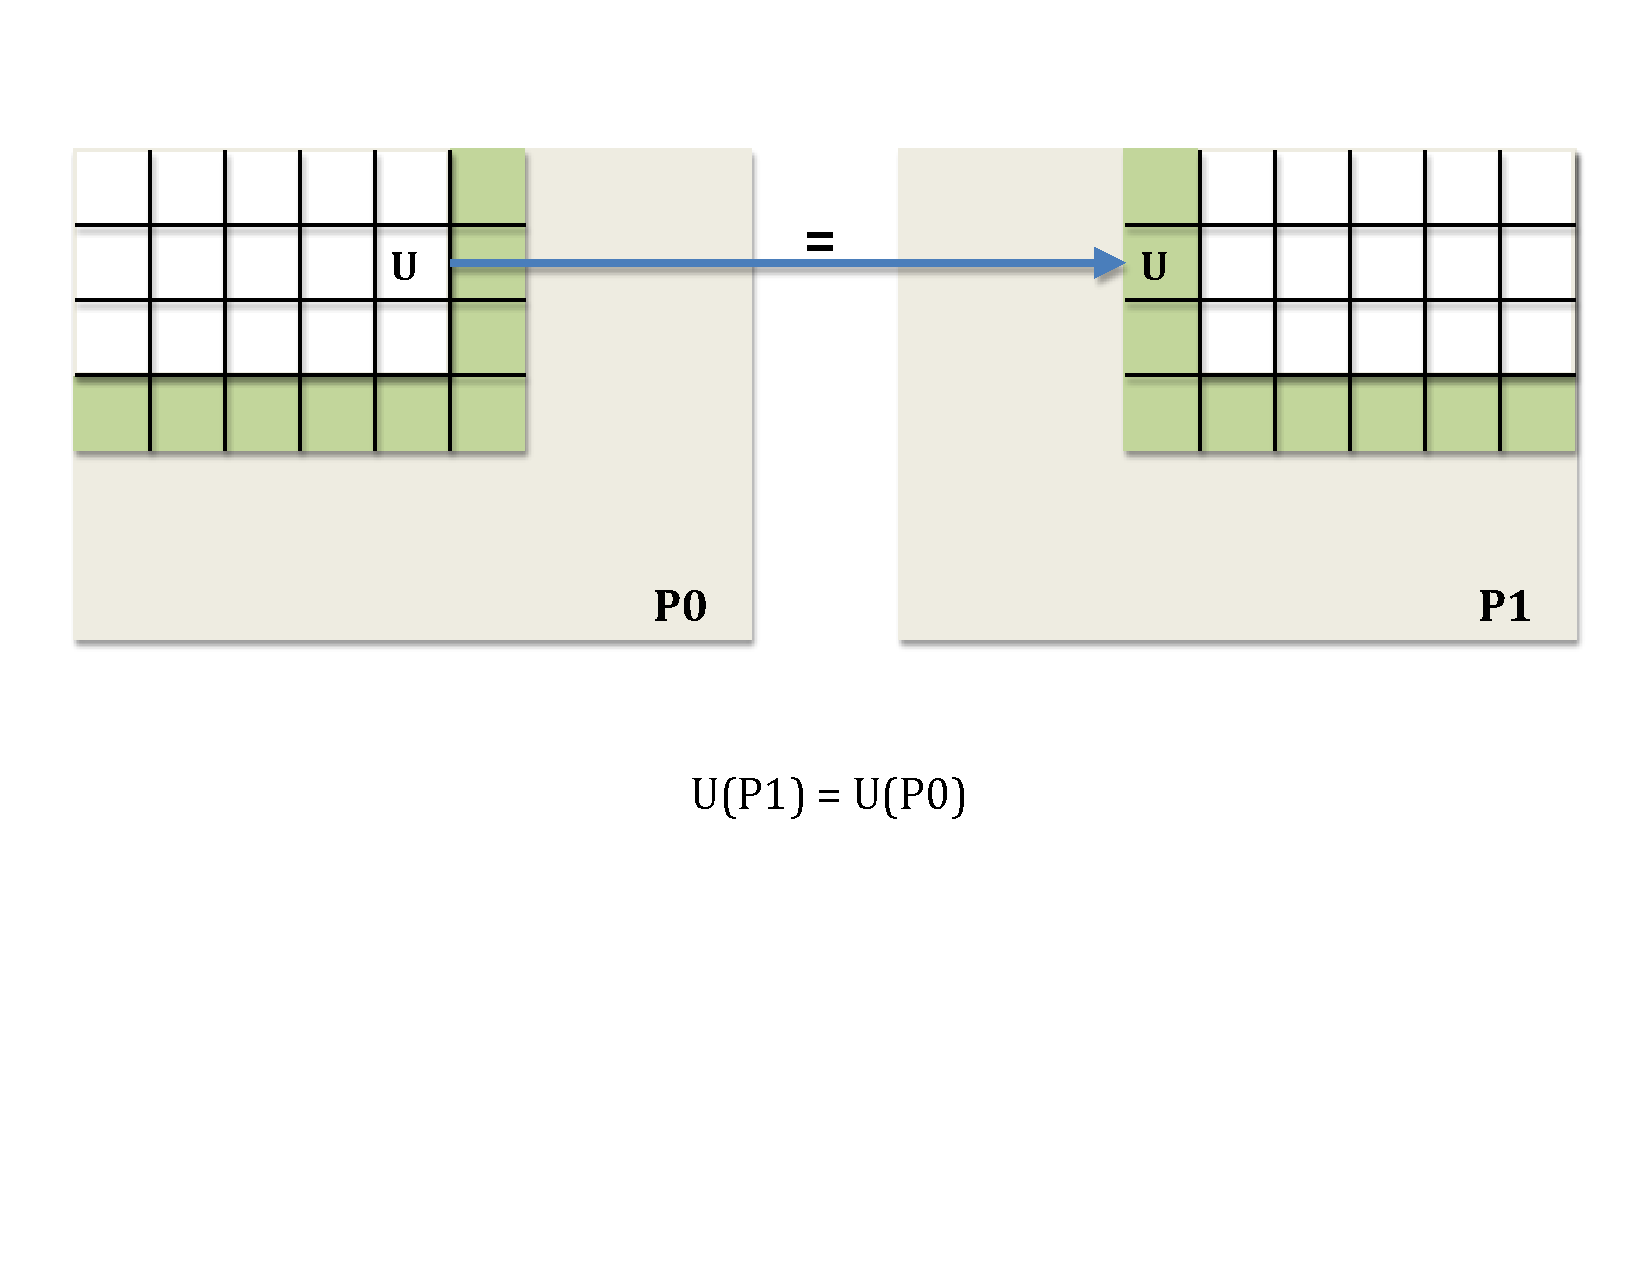
\includegraphics[trim=0cm 4cm 0cm 0cm, clip=true,width=0.8\textwidth]{fwm_mpi.pdf}
        }%
        \\
        \subfigure{%
           \label{fig:adm_mpi}
           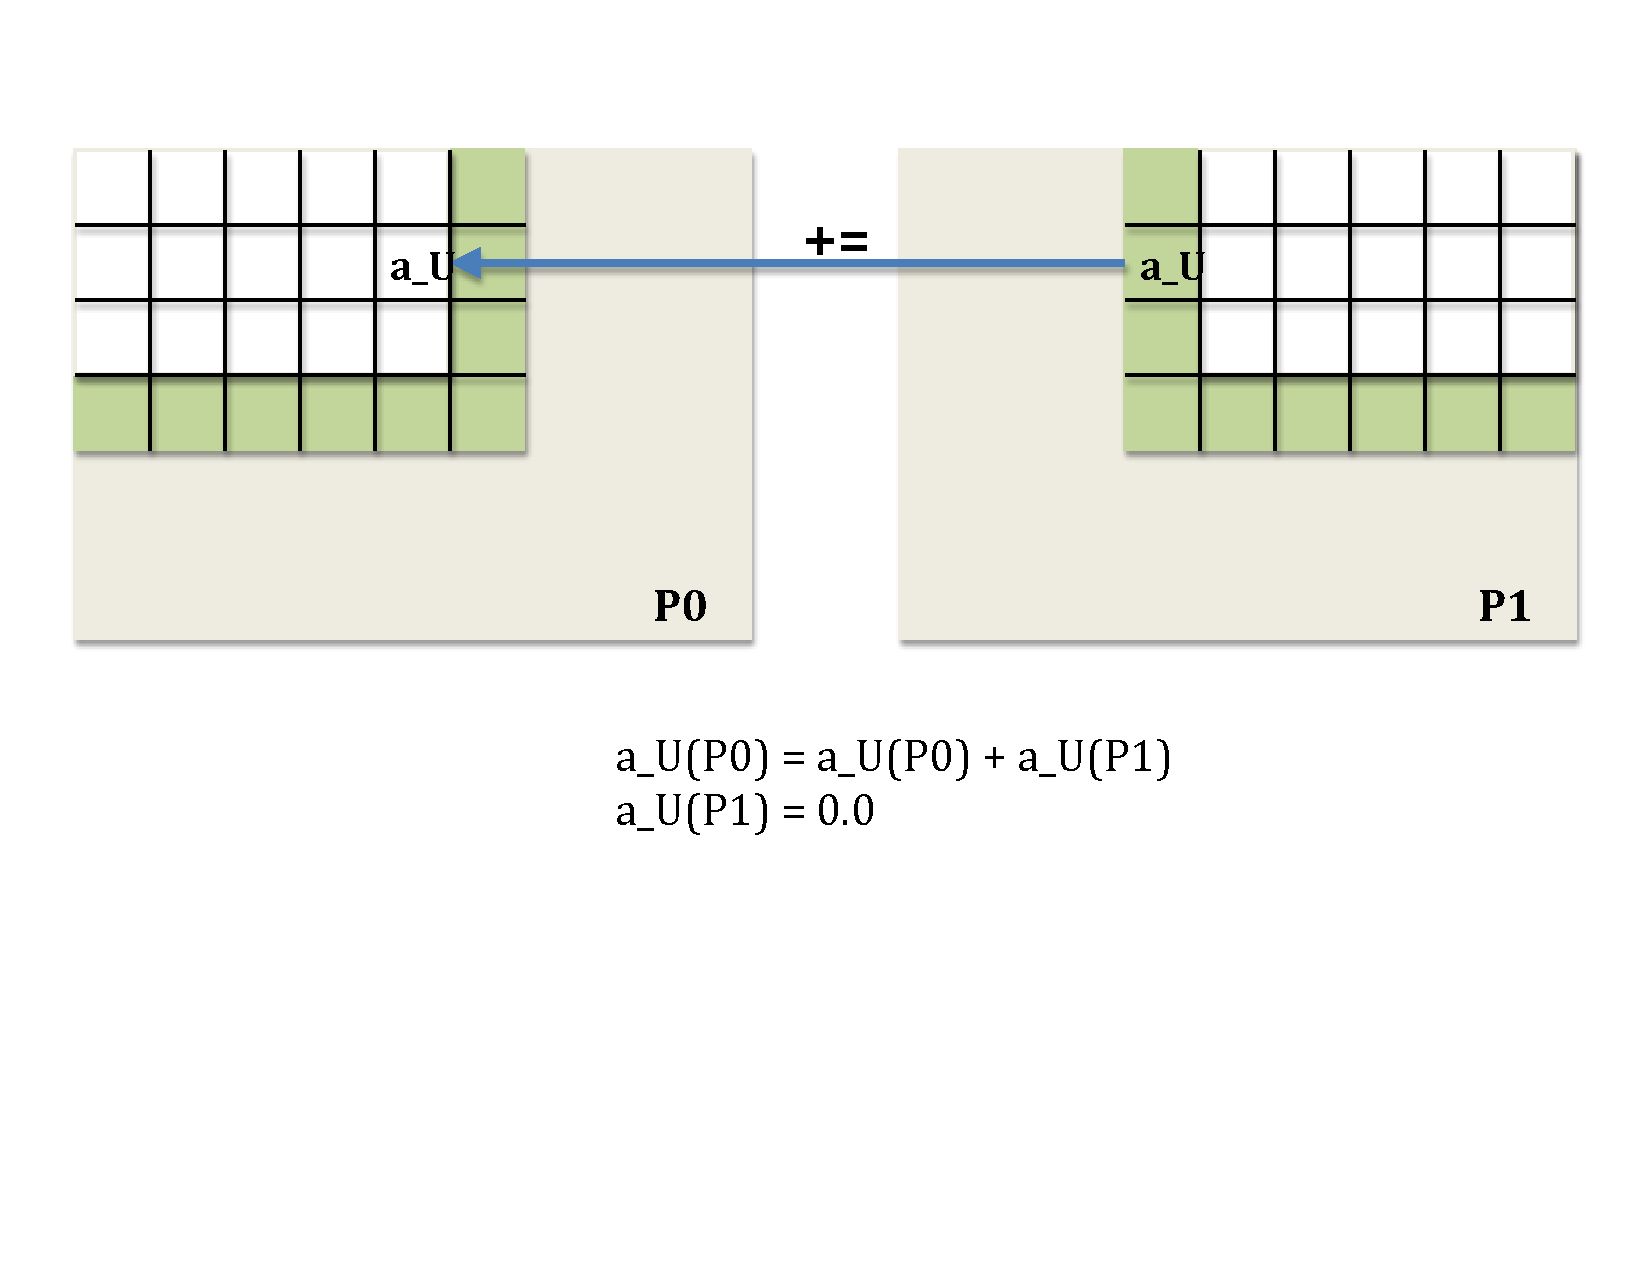
\includegraphics[trim=0cm 4cm 0cm 0cm, clip=true,width=0.8\textwidth]{adm_mpi.pdf}
        }\\ %  ------- End of the first row ----------------------%
%
    \end{center}
    \caption{%
        Schematic diagram for (a) halo exchange between two neighbor processors in FWM and (b) adjoint of halo exchange between two neighbor processors in ADM. Gray area denotes the entire model domain; Green zone denotes the ghost area; white zone is the computational patch for each processor; U denotes the basic state variable in the FWM and a\_U denotes the adjoint variable in the ADM.
     }%
   \label{fig:mpi}
\end{figure}

\begin{figure}[t]
     \begin{center}
%
        \subfigure{%
            \label{fig:bf_a}
            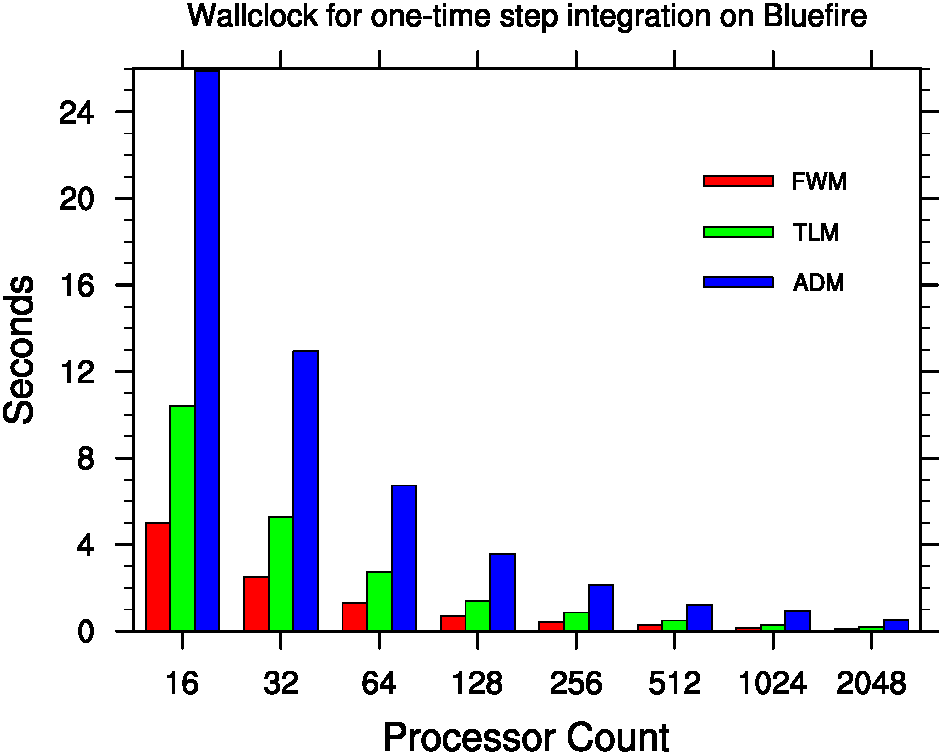
\includegraphics[width=0.7\textwidth]{bluefiretime.pdf}
        }%
        \\
        \subfigure{%
           \label{fig:bf_b}
           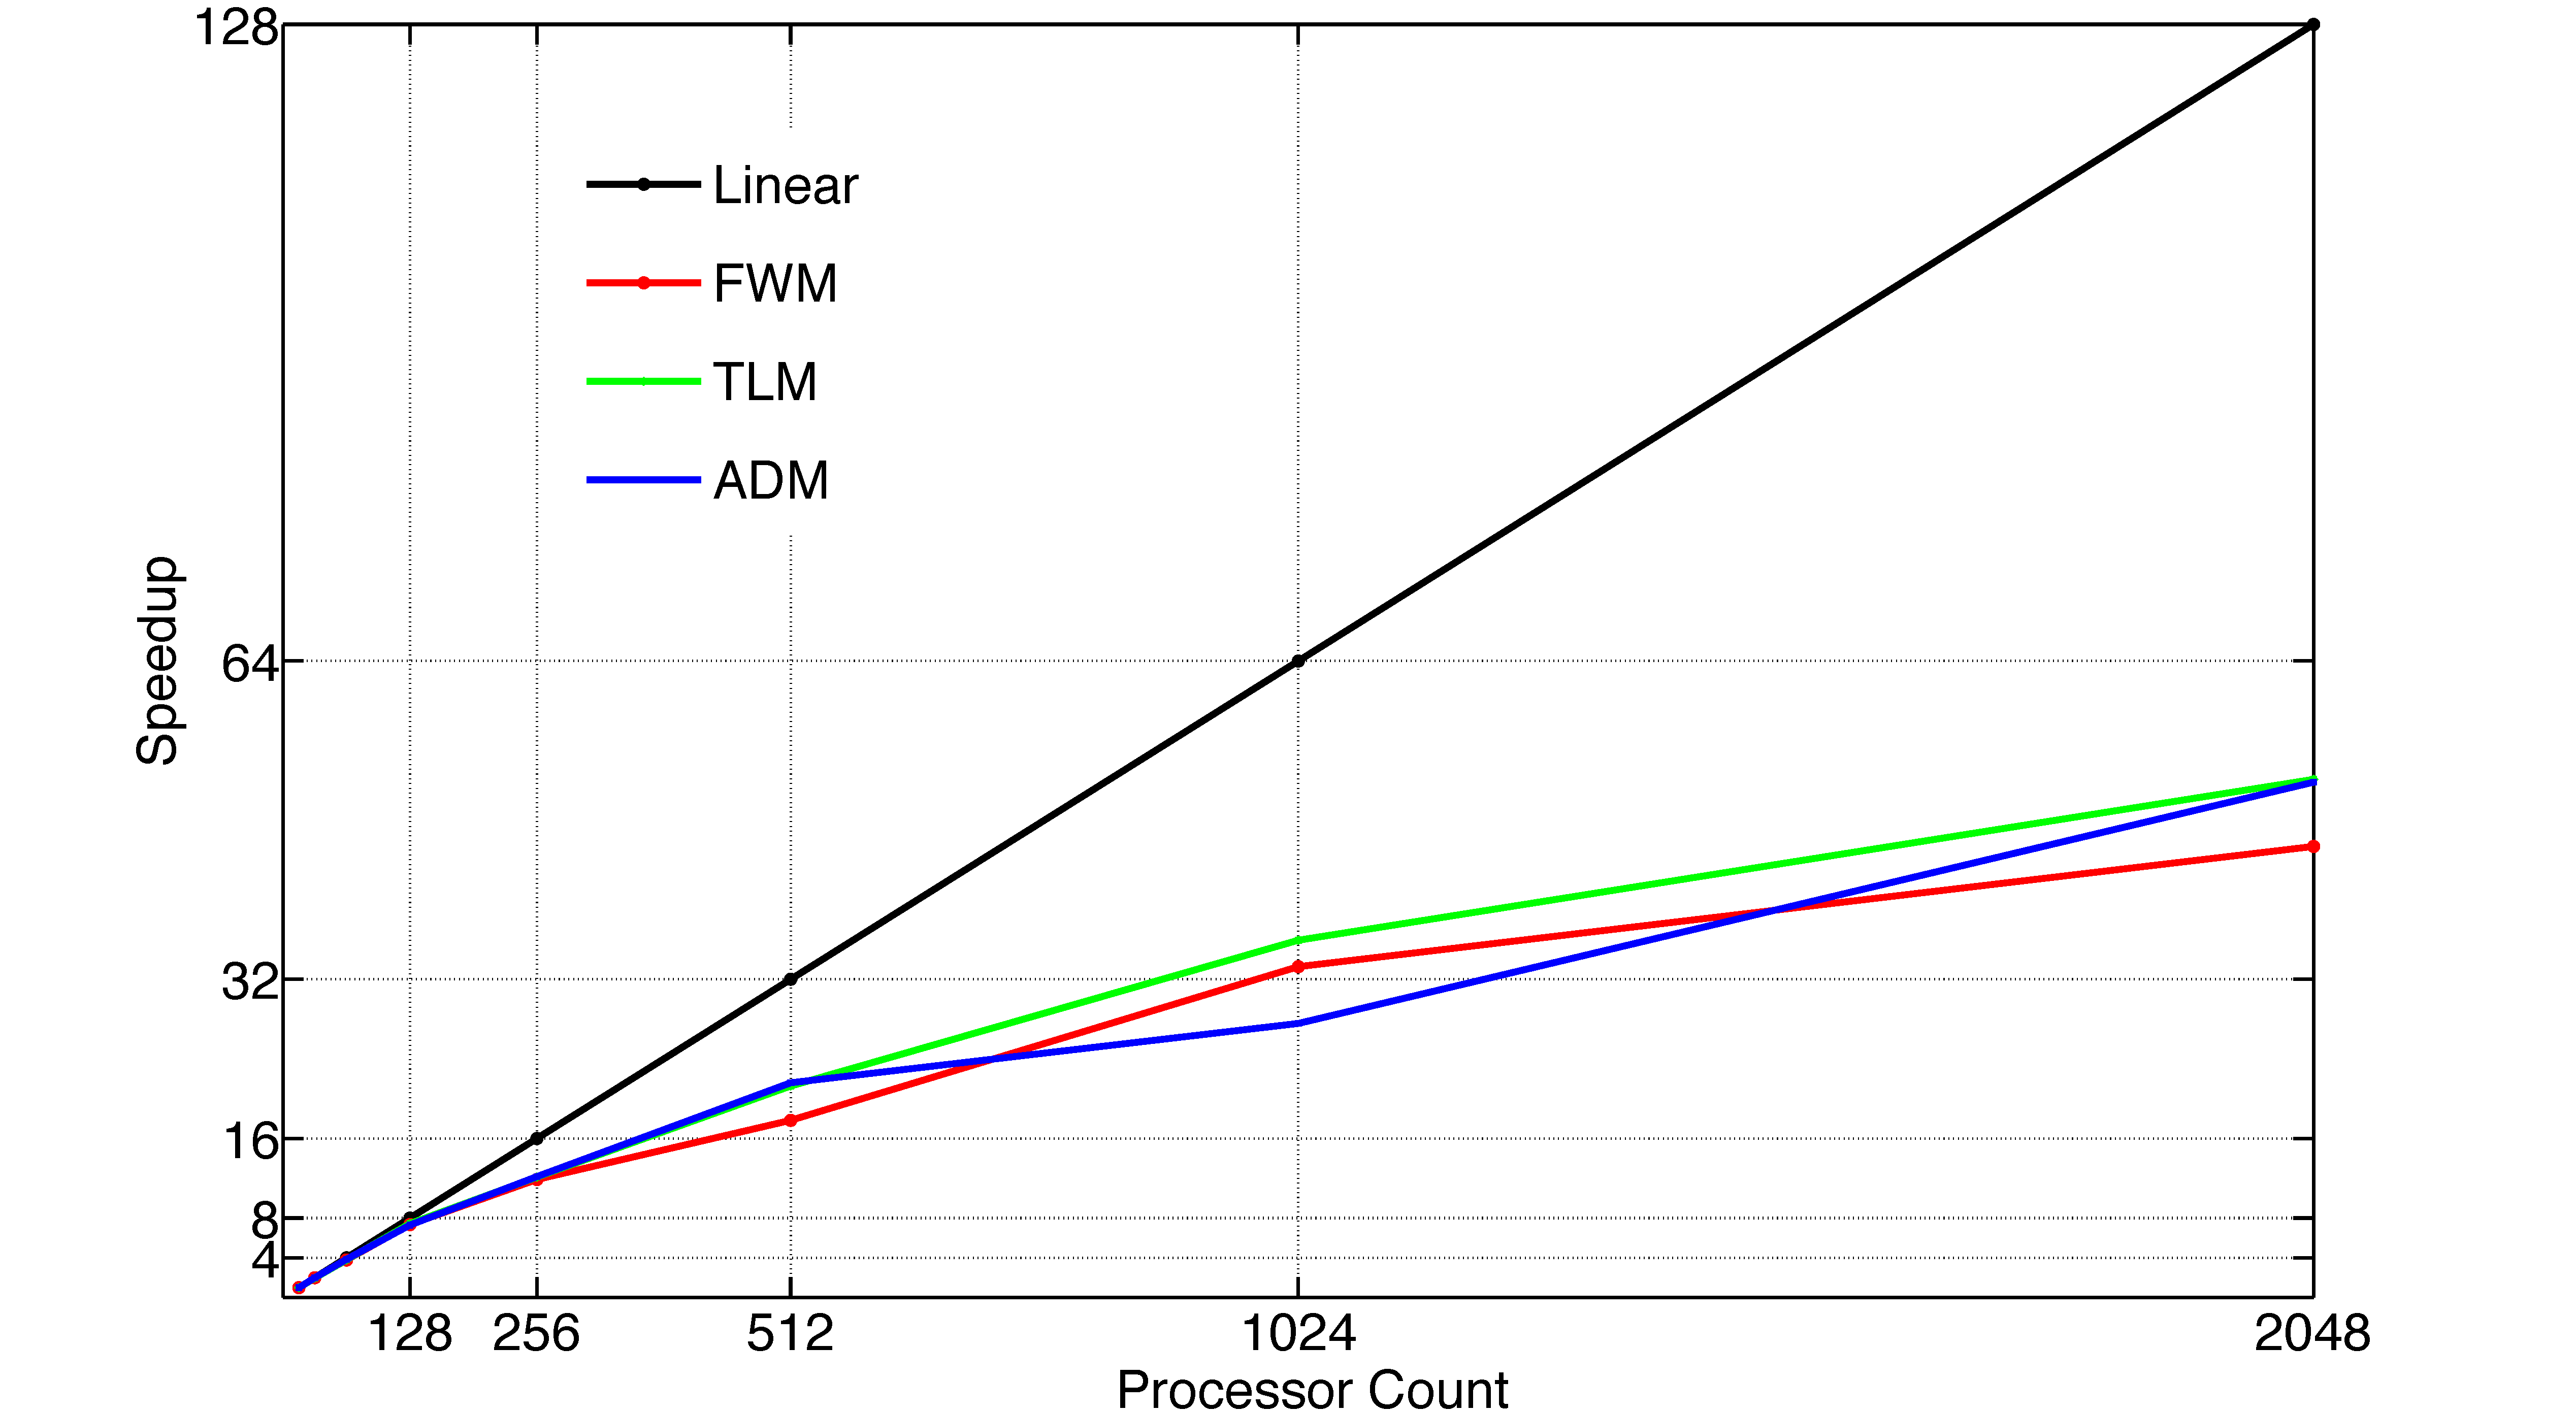
\includegraphics[width=0.8\textwidth]{bluefire_wrfplus_performance.pdf}
        }\\ %  ------- End of the first row ----------------------%
%
    \end{center}
    \caption{%
        Parallel performance for one-timestep integration on Bluefire in terms of (a) wallclock time and (b) parallel speedup.
     }%
   \label{fig:bluefire}
\end{figure}

\begin{figure}[t]
     \begin{center}
%
        \subfigure{%
            \label{fig:lx_a}
            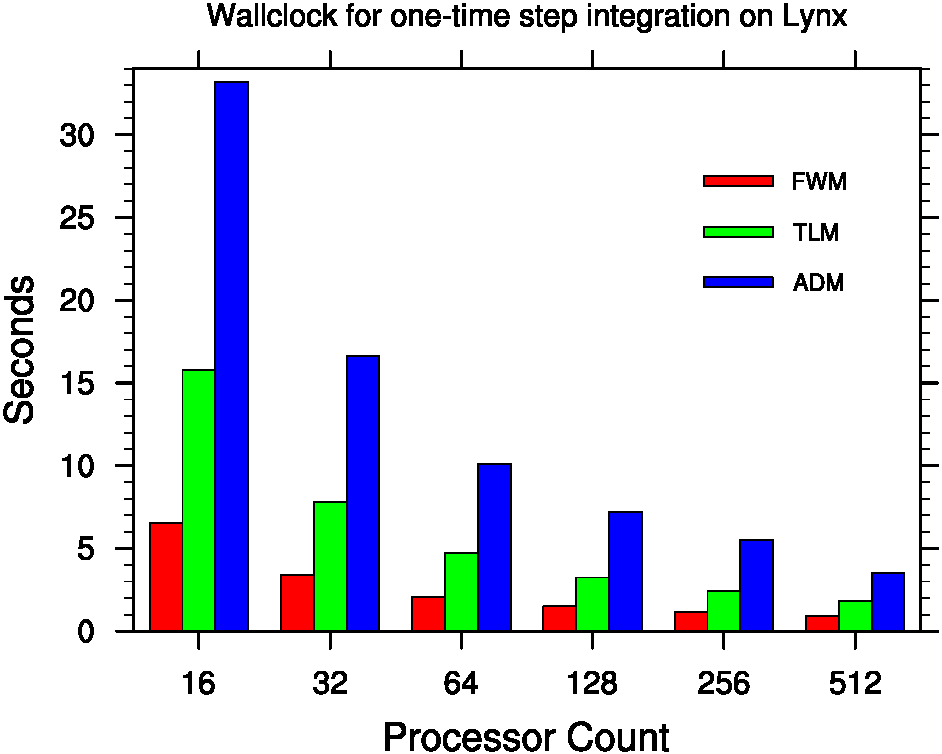
\includegraphics[width=0.7\textwidth]{lynxtime.pdf}
        }%
        \\
        \subfigure{%
           \label{fig:lx_b}
           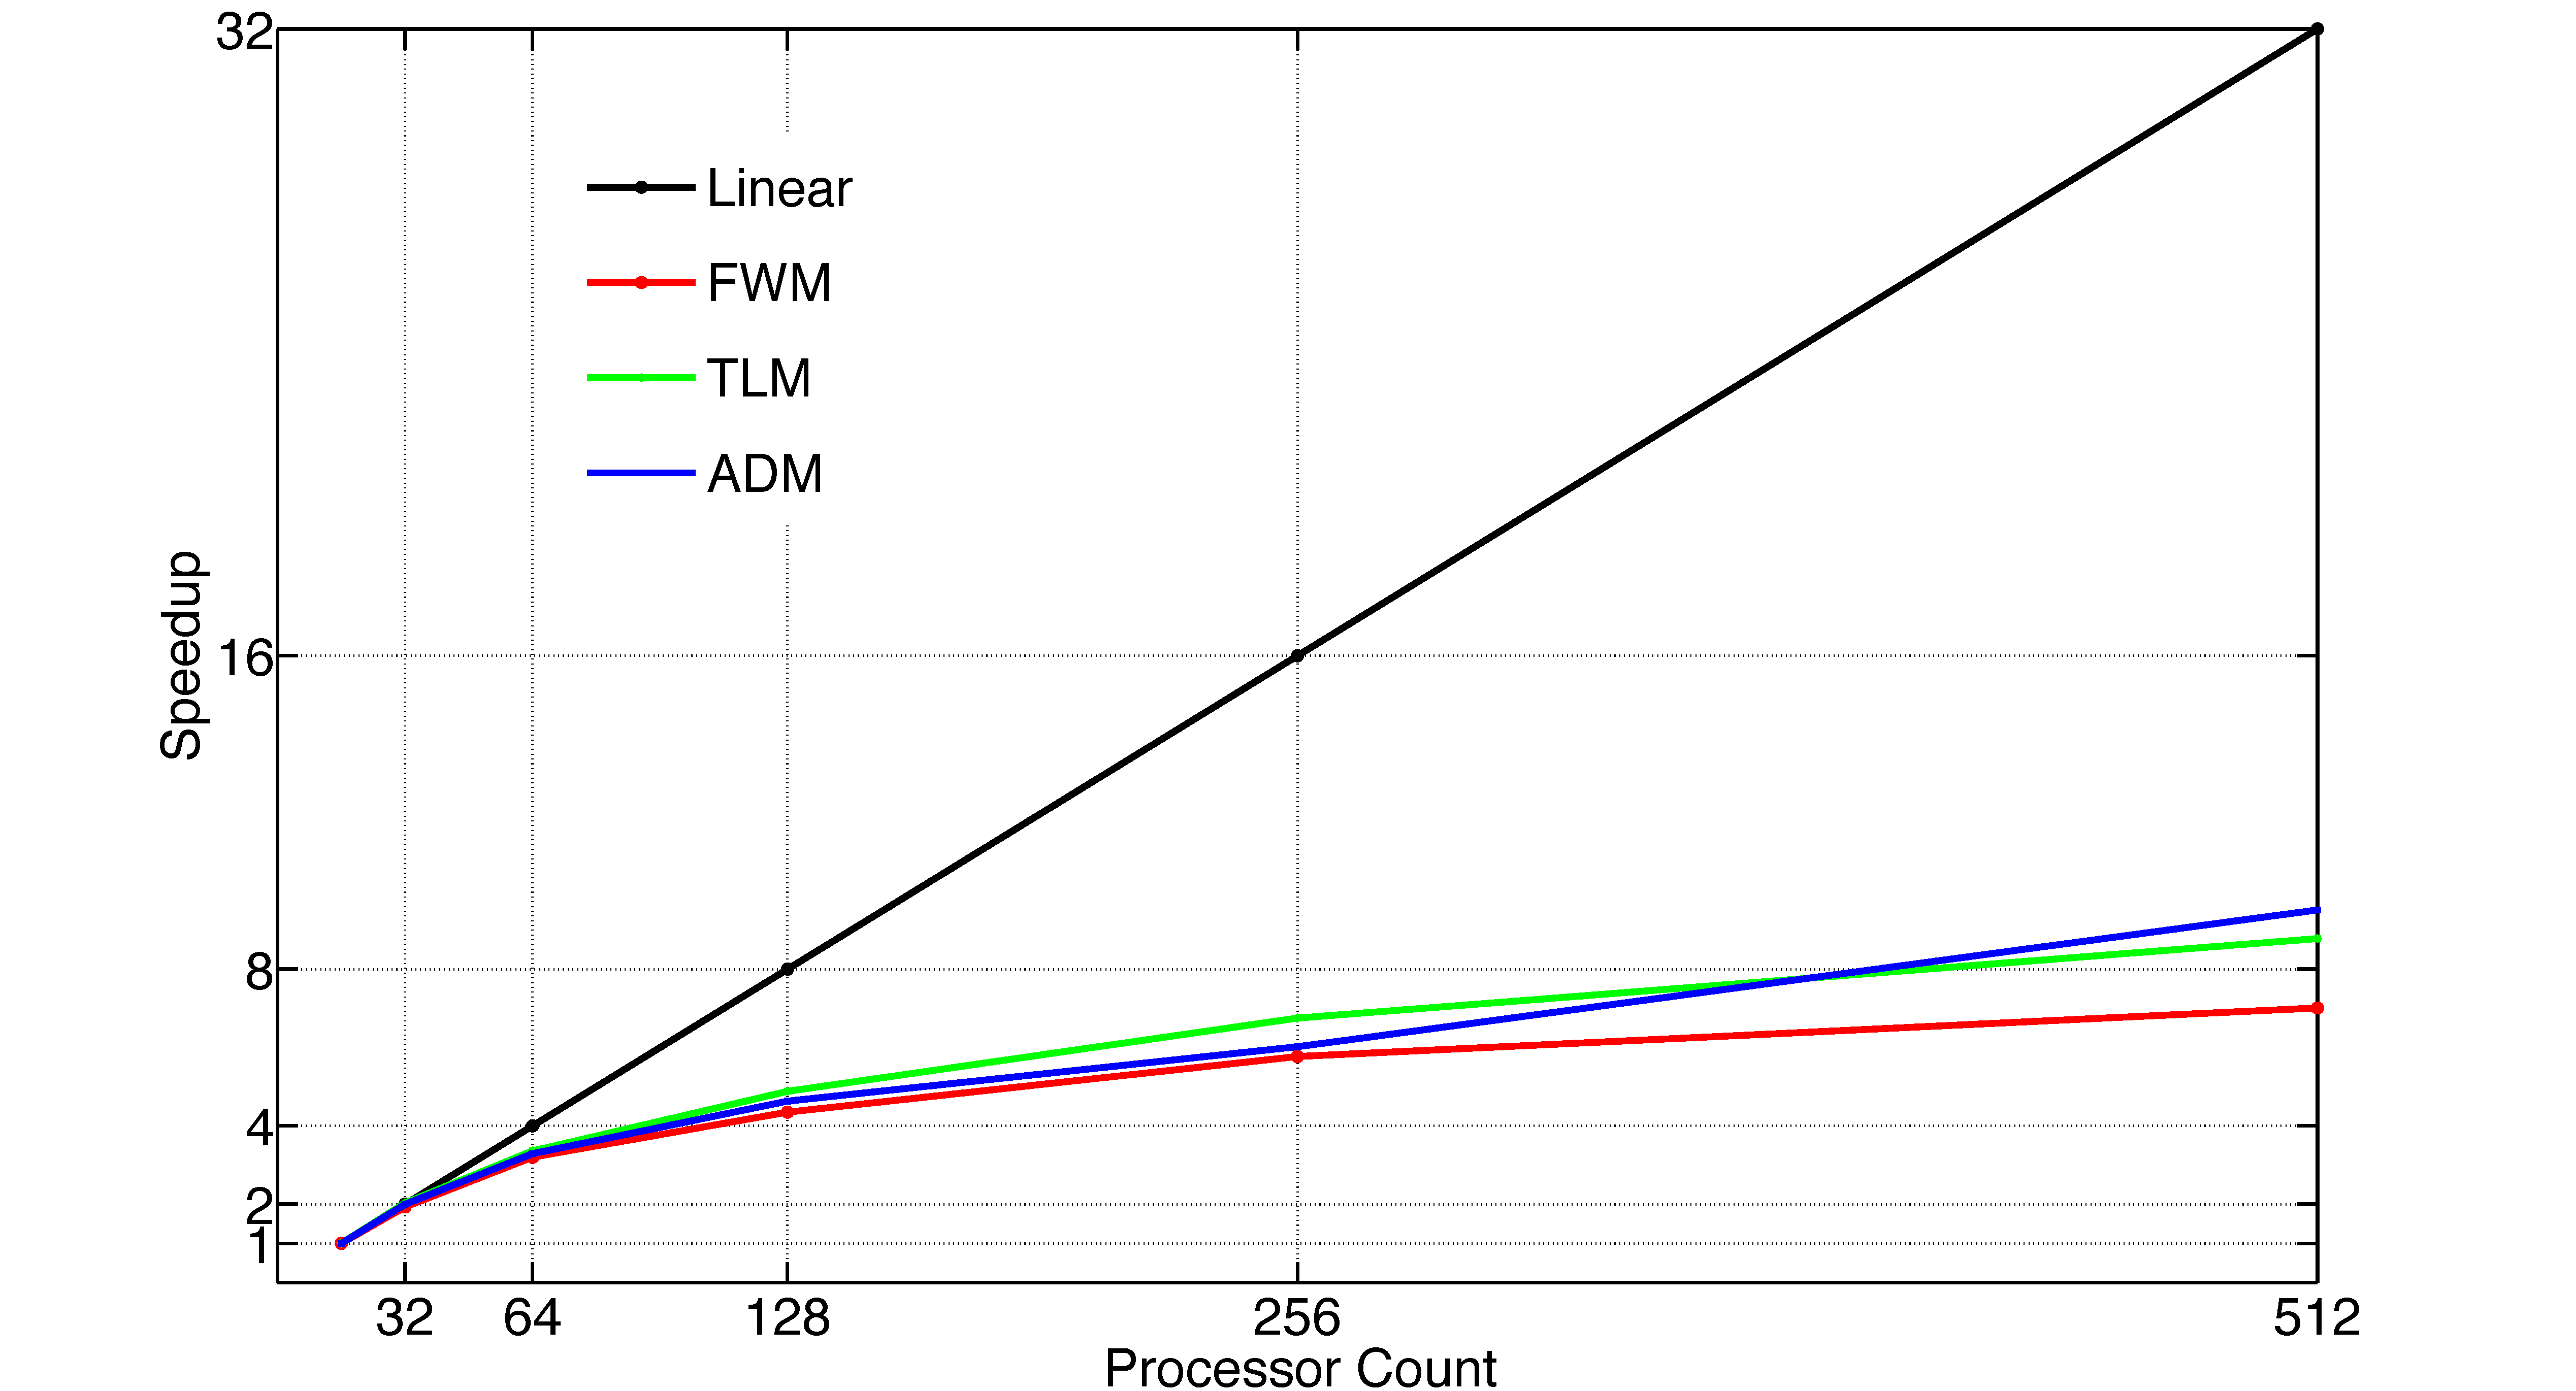
\includegraphics[width=0.8\textwidth]{lynx_wrfplus_performance.pdf}
        }\\ %  ------- End of the first row ----------------------%
%
    \end{center}
    \caption{%
        Parallel performance for one-timestep integration on Lynx in terms of (a) Wallclock time and (b) parallel speedup.
     }%
   \label{fig:lynx}
\end{figure}

\begin{figure}[t]
     \begin{center}
%
        \subfigure{%
            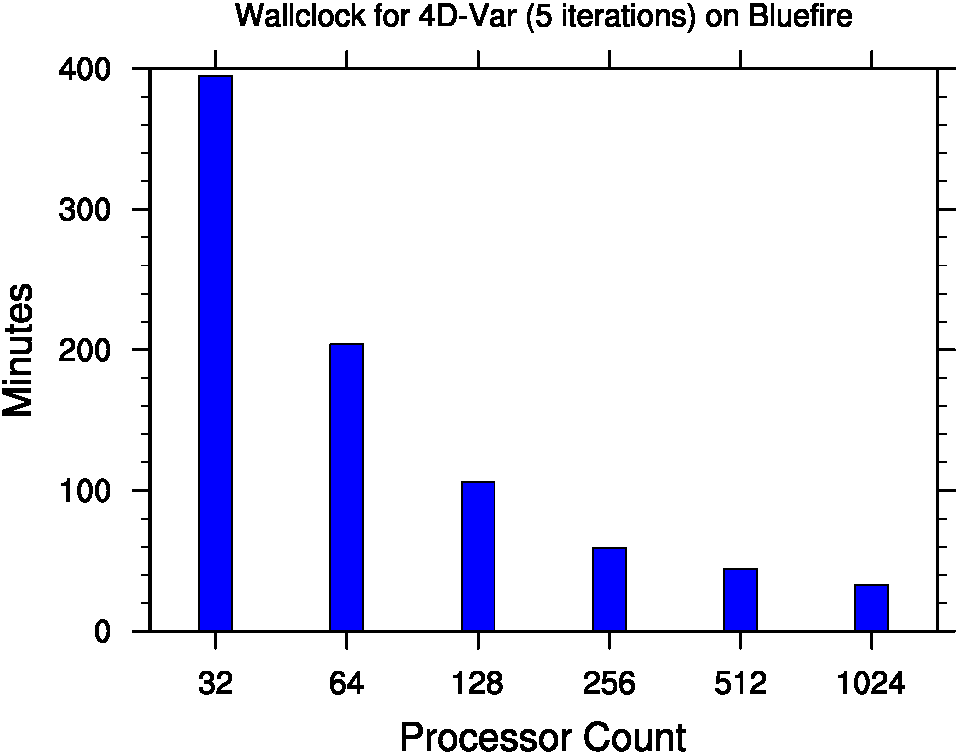
\includegraphics[width=0.7\textwidth]{4dvartime.pdf}
        }%
%
    \end{center}
    \caption{%
        Parallel performance for 4D-Var with 5 iterations on Bluefire
     }%
   \label{fig:4dvar}
\end{figure}


\subsection{Tables}
%%%%%%%%%%%%%%%%%%%%%%%%%%%%%%%%%%%%%%%%%%%%%%%%%%%%%%%%%%%%%%%%%%%%%
% TABLES
%%%%%%%%%%%%%%%%%%%%%%%%%%%%%%%%%%%%%%%%%%%%%%%%%%%%%%%%%%%%%%%%%%%%%
\begin{table}[t]
\caption{Ratio of norms between the tangent linear forecasts and the differences of the two nonlinear model forecasts at 24 h. The norm is defined as the summation of the squares of all variables (perturbations of tangent linear model and difference of two nonlinear models) over the whole domain at 24 h. Here $\lambda$ is the perturbation scaling factors of the initial perturbation.}\label{tlcheck}
\begin{center}
\begin{tabular}{cccccrcrc}
\hline\hline
$\lambda$ & $Ratio$ \\
\hline
.1000E+0 & 0.10114281198481E+01 \\
.1000E-01  & 0.10008545240448E+01 \\
.1000E-02  &  0.10000832484054E+01 \\
.1000E-03  &  0.10000095806229E+01 \\
.1000E-04  &  0.10000007503957E+01 \\
.1000E-05  &  0.10000001743469E+01 \\
.1000E-06  &  0.10000000344215E+01 \\
.1000E-07  &  0.99999998551913E+00 \\
.1000E-08  &  0.10000001453468E+01 \\
.1000E-09  &  0.10000007302081E+01 \\
.1000E-10  &  0.10000775631370E+01 \\
\hline
\end{tabular}
\end{center}
\end{table}


%\begin{table}[t]
%\caption{Parallel performance for one timestep integration on Bluefire: ${Wallclock}/{Speedup}$. $Linear$: Linear speedup; $FWM$: Forward model; $TLM$: Tangent linear model; $ADM$: Adjoint model.}\label{bluefire}
%\begin{center}
%\begin{tabular}{cccccrcrc}
%\hline\hline
%$Processors$ & $Linear$ & $FWM$ & $TLM$ & $ADM$ \\
%\hline
%16 & 1 & 4.99s/1.0 & 10.42s/1.0 & 25.91s/1.0 \\
%32 & 2 & 2.49s/2.0 & 5.28s/1.97 & 12.93s/2.0 \\
%64 & 4 & 1.32s/3.78 & 2.74s/3.80 & 6.73s/3.85 \\
%128 & 8 & 0.68s/7.34 & 1.40s/7.44 & 3.55s/7.30 \\
%256 & 16 & 0.42s/11.88 & 0.86s/12.12 & 2.13s/12.16 \\
%512 & 32 & 0.28s/17.82 & 0.49s/21.27 & 1.20s/21.60 \\
%1024 & 64 & 0.15s/33.27 & 0.29s/35.93 & 0.94s/27.56 \\
%2048 & 128 & 0.11s/45.36 & 0.20s/52.10 & 0.50s/51.82 \\
%\hline
%\end{tabular}
%\end{center}
%\end{table}

%
%\begin{table}[t]
%\caption{Parallel performance for one timestep integration on Lynx: ${Wallclock}/{Speedup}$. $Linear$: Linear speedup; $FWM$: Forward model; $TLM$: Tangent linear model; $ADM$: Adjoint model..}\label{lynx}
%\begin{center}
%\begin{tabular}{cccccrcrc}
%\hline\hline
%$Processors$ & $Linear$ & $FWM$ & $TLM$ & $ADM$ \\
%\hline
%16 & 1 & 6.52s/1.0 & 15.80s/1.0 & 33.20s/1.0 \\
%32 & 2  & 3.37s/1.93  & 7.78s/2.03 & 16.63s/2.0 \\
%64 & 4 & 2.04s/3.20 & 4.70s/3.36 & 10.12s/3.29 \\
%128 & 8 & 1.50s/4.35 & 3.24s/4.88 & 7.20s/4.63 \\
%256 & 16 & 1.13s/5.77 & 2.43s/6.75 & 5.53s/6.02 \\
%512 & 32 & 0.93s/7.01 & 1.80s/8.78 & 3.50s/9.51 \\
%\hline
%\end{tabular}
%\end{center}
%\end{table}

%%%%%%%%%%%%%%%%%%%%%%%%%%%%%%%%%%%%%%%%%%%%%%%%%%%%%%%%%%%%%%%%%%%%%
% ACKNOWLEDGMENTS
%%%%%%%%%%%%%%%%%%%%%%%%%%%%%%%%%%%%%%%%%%%%%%%%%%%%%%%%%%%%%%%%%%%%%

\begin{acknowledgment}
The National Center for Atmospheric Research is sponsored by the National
Science Foundation.  This work is supported by the Air Force Weather Agency. The WRFPLUS system benefitted greatly from close collaboration with Dr. Qiang Chen and his Adjoint Code Generator. We thank Dong-Kyou Lee and Gyu-Ho Lim of Seoul National University for their comments on the manuscript and generous support through Korea-USA Weather and Climate Center. We thank Fuqing Zhang and Jon Poterjoy of Penn State University for their valuable suggestions and comments on the manuscript. Mary Golden helped to edit the manuscript.
\end{acknowledgment}


%%%%%%%%%%%%%%%%%%%%%%%%%%%%%%%%%%%%%%%%%%%%%%%%%%%%%%%%%%%%%%%%%%%%%
% REFERENCES
%%%%%%%%%%%%%%%%%%%%%%%%%%%%%%%%%%%%%%%%%%%%%%%%%%%%%%%%%%%%%%%%%%%%%
% Create a bibliography directory and place your .bib file there.
\ifthenelse{\boolean{dc}}
{}
{\clearpage}
\bibliographystyle{ametsoc}
%\bibliography{../bibliography/references}
\bibliography{references}
\end{document}
%%%%%%%%%%%%%%%%%%%%%%%%%%%%%%%%%%%%%%%%%%%%%%%%%%%%%%%%%%%%%%%%%%%%%
% END OF TEMPLATE
%%%%%%%%%%%%%%%%%%%%%%%%%%%%%%%%%%%%%%%%%%%%%%%%%%%%%%%%%%%%%%%%%%%%%
